%!TEX root = ../main.tex

\subsection{Normal component}\label{ss:normal_component}
% What?
This section discusses the parametrization of both the `fake' and `real' normals. We differentiate between these two normal types because originally point-normal triangles normals are interpolated based on a quadratic patch, the `fake' normals (see \crefs{sss:method:normals:fakeNormals}), whereas one would get the `real' normals by calculating them based on the actual surface (see \crefs{sss:method:normals:realNormals}).

It should be noted that, just as with the geometric component, the normal component of the point-normal triangle is computed solely based on the input primitive, i.e., the vertex positions and their normals, as shown in \cref{fig:method:input_primitive}. 

\begin{figure}
	\centering
	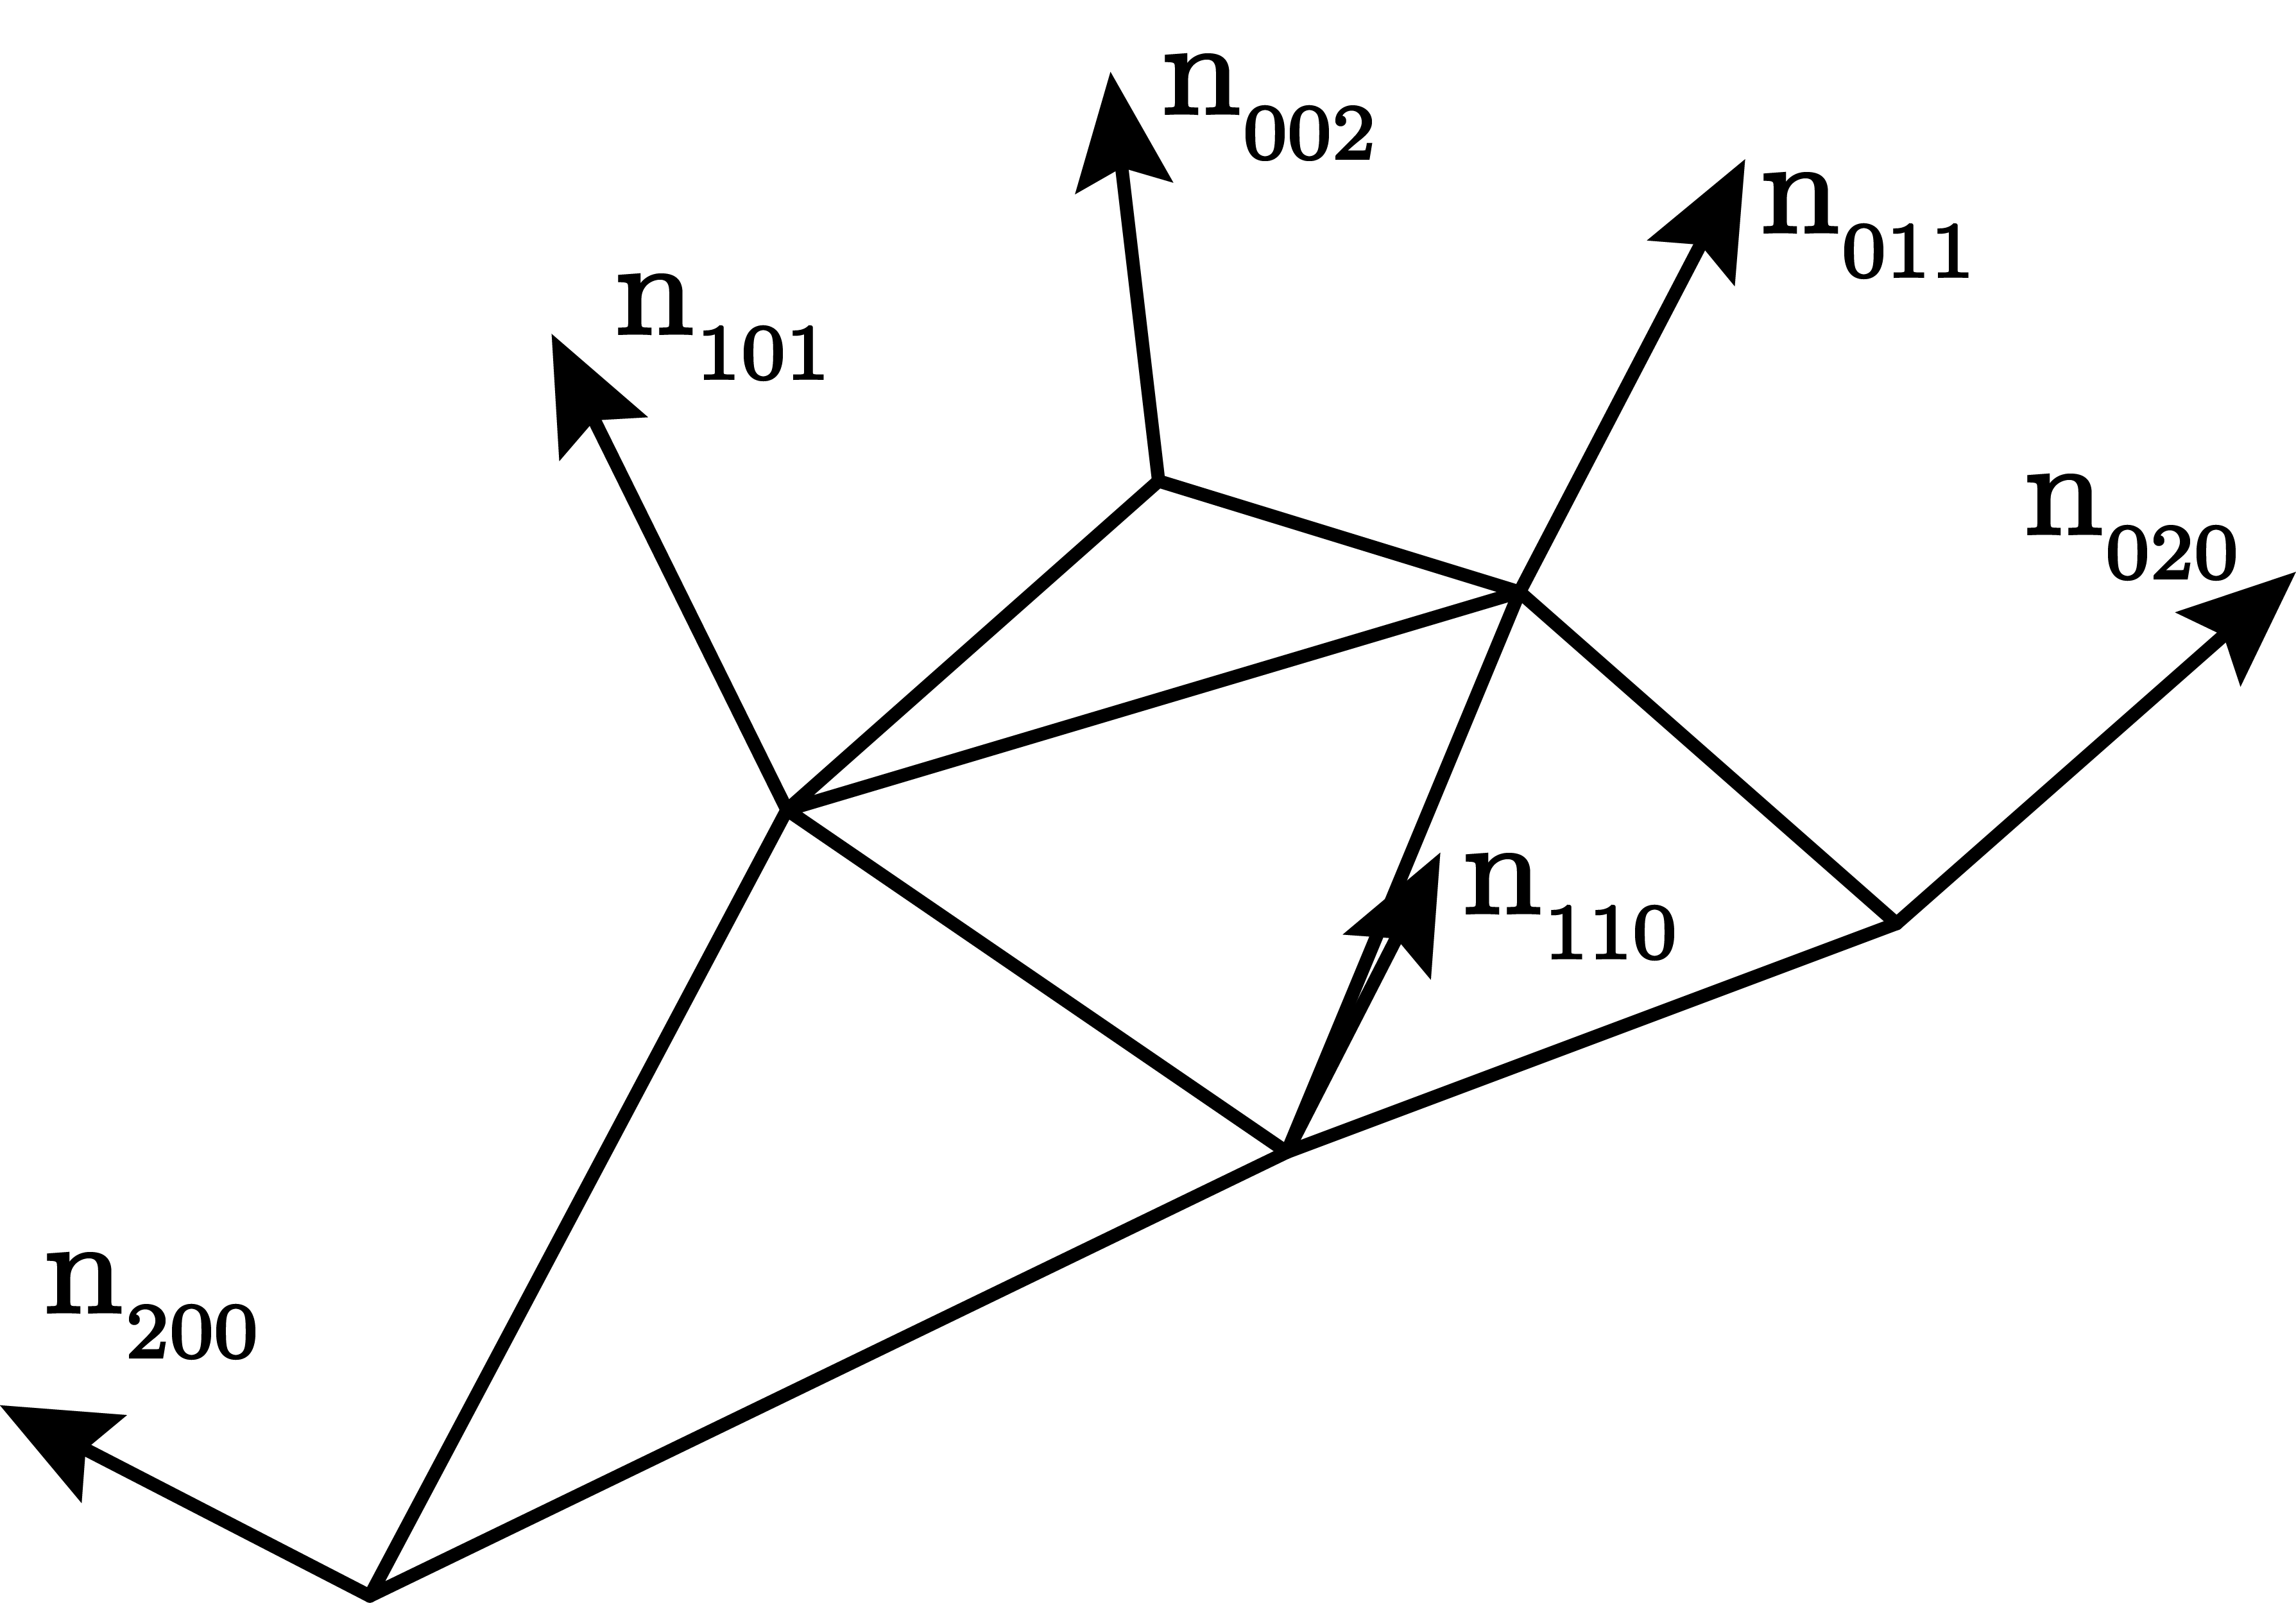
\includegraphics[width=0.45\textwidth]{./content/img/method/normals.png}
	\caption{The normal field of the point-normal triangle.}
	\label{fig:method:normal_field}
\end{figure}

\subsubsection{Fake normals}
\label{sss:method:normals:fakeNormals}
	\citeauthor{vlachos2001curved} define the `fake' normals using a quadratic function $n(u,v)$:
	\begin{align}
	\noalign{$n(u,v): \quad R^2 \mapsto R^3,\quad$ for $w = 1 - u - v, \quad u, v, w \geq 0$}
	\begin{split}\label{eq:method:quadratic_normal_patch}
	    n(u,v) ={}& \sum_{i + j + k = 2} n_{ijk}u^i v^j w^k,\\
	      	   ={}& n_{200}w^2 + n_{020}u^2 + n_{002}v^2\\
	      	    {}& + n_{110}wu + n_{011}uv + n_{101}wv\\
	\end{split}
	\end{align}
	The coefficients of this quadratic `patch' are the normals shown in \cref{fig:method:normal_field}. The normals are computed for a point, halfway on every edge, i.e., $(u,v,w) = (\frac{1}{2}, \frac{1}{2}, 0)$, $(0, \frac{1}{2}, \frac{1}{2})$, $(\frac{1}{2}, 0, \frac{1}{2})$. Point-normal triangles use quadratically varying normals to be able to capture the inflection points that are possible due to the cubic geometric component. 

	\Cref{fig:method:linear_vs_quadratically_varying} illustrates why one needs quadratic patches to capture these inflection points. \Cref{fig:method:linear_vs_quadratically_varying} illustrates two cases: \cref{fig:method:normal:both} shows that when the normals point in a different direction the surface will be parabolic, and no inflection point exists. In this case both linear and quadratically varying normals are able to capture the surface. In \cref{fig:method:normal:linear} and \cref{fig:method:normal:quadratic} the case were an inflection point exists is shown. We see that (\cref{fig:method:normal:linear}) linear varying normals do not capture the inflection point, i.e., give incorrect normals. The quadratically varying normals do give the correct normals (\cref{fig:method:normal:quadratic}), i.e, they capture the inflection point.

	\begin{figure}
		\centering
		\begin{subfigure}{\columnwidth}
			\centering
			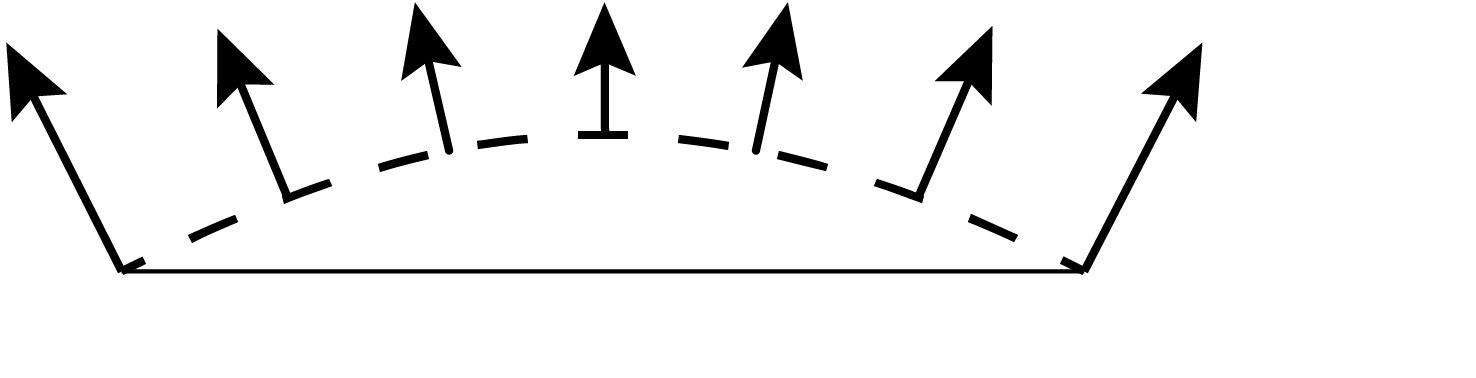
\includegraphics[width=0.8\textwidth]{./content/img/method/linearVsQuadraticNormals_both.png}
			\caption{Vector averaging with either linear or quadratic over a curve without inflections.}
			\label{fig:method:normal:both}
		\end{subfigure}
		\begin{subfigure}{\columnwidth}
			\centering
			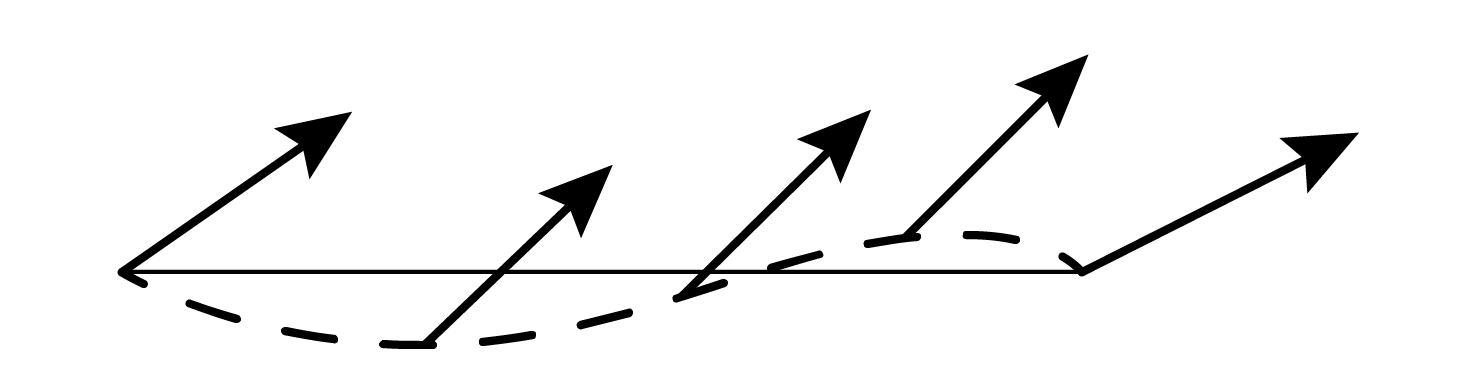
\includegraphics[width=0.8\textwidth]{./content/img/method/linearVsQuadraticNormals_linear}
			\caption{Vector averaging with linear interpolation over a curve with an inflection.}
			\label{fig:method:normal:linear}
		\end{subfigure}	
		\begin{subfigure}{\columnwidth}
			\centering
			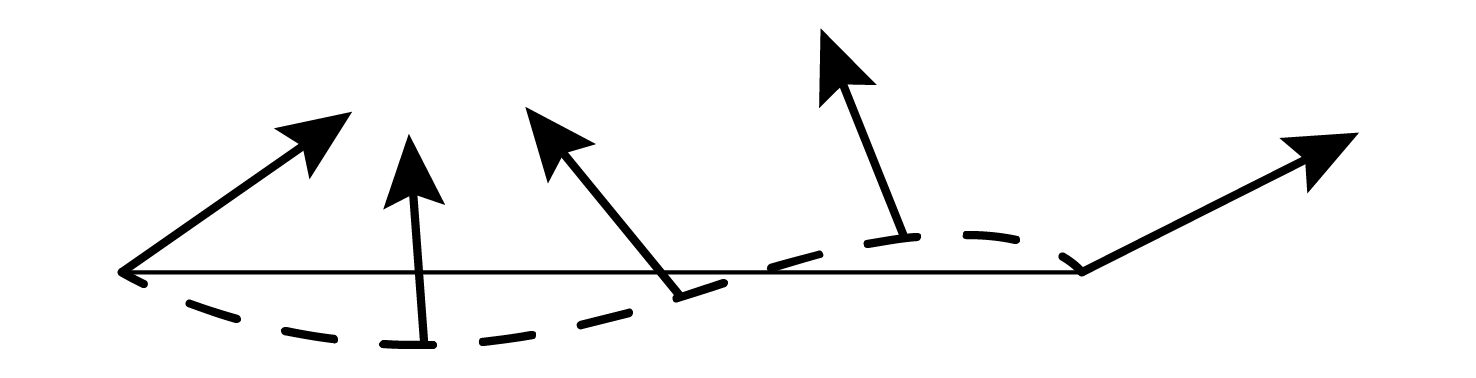
\includegraphics[width=0.8\textwidth]{./content/img/method/linearVsQuadraticNormals_quadratic}
			\caption{Vector averaging with quadratic interpolation over a curve with an inflection.}
			\label{fig:method:normal:quadratic}
		\end{subfigure}			
		\caption{Examples of normal vector averaging over an edge. The dashed lines indicate the profile of the surface that should be approximated. The normals of a curves without inflections are correctly approximated by both linear and quadratic interpolation, see \cref{fig:method:normal:both}. The normals of a curve with inflections are incorrectly approximated with \subref{fig:method:normal:linear} linear interpolation and correctly with \subref{fig:method:normal:quadratic} interpolation. Image \subref{fig:method:normal:both} was adapted from \cite{van1997phong}, image \subref{fig:method:normal:linear} and \subref{fig:method:normal:quadratic} from \cite{vlachos2001curved}.}
		\label{fig:method:linear_vs_quadratically_varying}
	\end{figure}

	\todo[inline]{Discuss parametrization of `quadratic' patch}

	Using the function $n(u,v)$, see \eqref{eq:method:quadratic_normal_patch}, the normal of any point parametrized by the barycentric coordinates $(u,v)$ can be calculated. To do this we first need to define a control net. We consider two different types of coefficients: the vertex normals, $n_{200}$, $n_{020}$, and $n_{002}$; and the edge normals, $n_{110}$, $n_{011}$, and $n_{101}$.
	\todo[inline]{Discuss the construction of the control points for the `quadratic' patch}

	An edge normal is calculated by taking the average of the two input vertex normals of the vertices of the edge. After this step this looks like the image shown in \cref{fig:method:normal:linear}. To capture the inflection point the average normal is then reflected across the plane perpendicular to the edge, see \cref{fig:method:normal:reflection}. When a inflection point exists this will give the correct mid-edge normal (see \cref{fig:method:normal:quadratic}) and this will also not alter the normal field if no inflection point is present, e.g., imagine reflecting the mid-edge normal of the curve shown in \cref{fig:method:normal:both}, this will result in the same normals.

	\begin{figure}
		\centering
		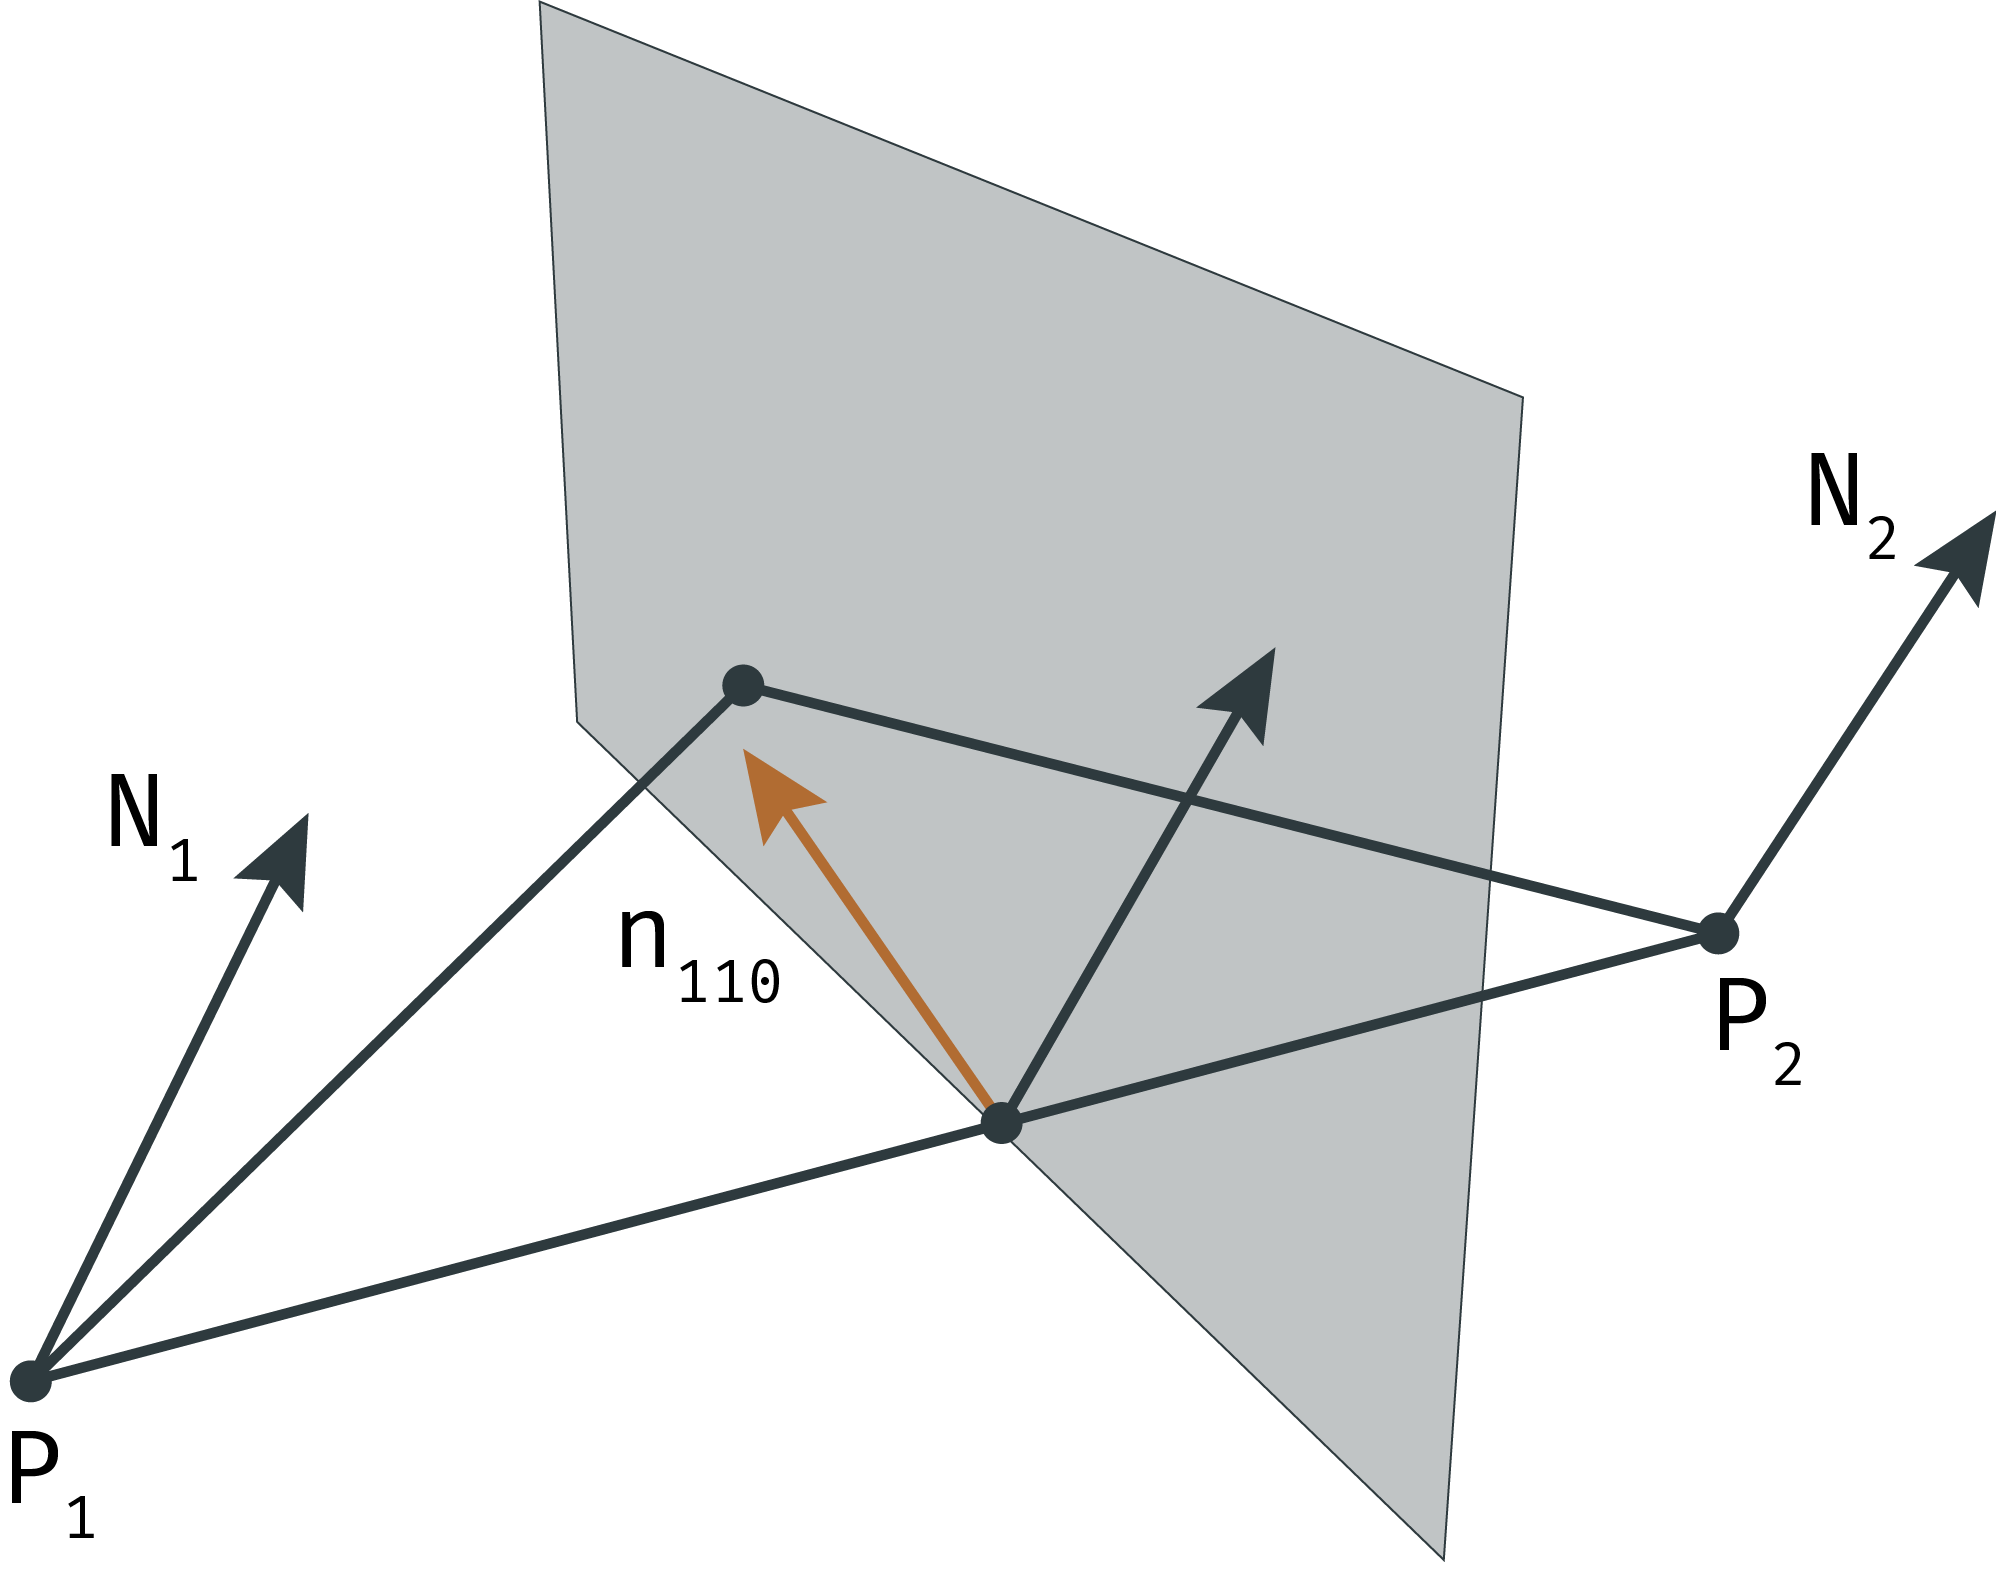
\includegraphics[width=0.45\textwidth]{./content/img/method/normal_reflection.png}
		\caption{Construction of the mid-edge normal coefficient, used for quadratically varying normals. The two input normals are averaged and then reflected reflected across the plane perpendicular to the edge.}
		\label{fig:method:normal:reflection}
	\end{figure}

	The vertex normals are simply the normals provided by the input primitive.

\subsubsection{Real normals}
\label{sss:method:normals:realNormals}
		\todo[inline]{Discuss how to compute the real normals given the geometric component}
		The real normals are computed based on the geometric component of the point-normal triangle. This is done by taking the cross product of the the partial derivatives with respect to $u$ and $v$. For the partial derivatives with respect to $u$ and $v$ see \eqref{eq:method:normal:partialU} and \eqref{eq:method:normal:partialV} respectively.

		\begin{align} \label{eq:method:normal:partialU}
			\frac{\partial b(u,v)}{\partial u} ={}& \sum_{i + j + k = 2} b_{i+1, j, k} \frac{2!}{i!j!k!} u^i v^j w^k  \nonumber\\
										   ={}& w^2 b_{102} + v^2 b_{120} + u^2 b_{300} + \\
										    {}& 2 v w b_{111} + 2 u w b_{201} + 2 u v b_{210} \nonumber 
		\end{align}

		\begin{align} \label{eq:method:normal:partialV}
			\frac{\partial b(u,v)}{\partial v} ={}& \sum_{i + j + k = 2} b_{i, j + 1, k} \frac{2!}{i!j!k!}u^i v^j w^k \nonumber \\
											   ={}& w^2 b_{012} + v^2 b_{030} + u^2 b_{210} + \\
											    {}& 2 v w b_{021} + 2 u w b_{111} + 2 u v b_{120} \nonumber
		\end{align}

		The partial derivatives in \eqref{eq:method:normal:partialU} and \eqref{eq:method:normal:partialV} define two tangent vectors in the $u$ and $v$ directions, at a point $(u,v)$ of the surface. By taking the crossproduct of these two vectors, at a point, we find the `real' normal of that point defined by the geometric component of the point-normal triangle.